\documentclass[12pt]{beamer}
\usepackage{color}
\usepackage[T2A]{fontenc}
\usepackage{colordvi}
\usepackage{../../MyPackages/commands}
\usepackage[absolute,overlay]{textpos}
\usepackage{setspace}

\defbeamertemplate{footline}{centered page number}
{%
  \hspace*{\fill}%
  \usebeamercolor[fg]{page number in head/foot}%
  \usebeamerfont{page number in head/foot}%
  \insertpagenumber\,/\,\insertpresentationendpage%
  \hspace*{\fill}\vskip2pt%
}
\setbeamertemplate{footline}[centered page number]
%\mode<presentation>{
%\usetheme{Rochester}
%}

\mode<presentation>{
  \usetheme{AnnArbor}
}
\makeatletter
\setbeamertemplate{footline}
{
  \leavevmode%
  \hbox{%
  \begin{beamercolorbox}[wd=.333333\paperwidth,ht=2.25ex,dp=1ex,center]{author in head/foot}%
    \usebeamerfont{author in head/foot}\insertshortauthor%~~\beamer@ifempty{\insertshortinstitute}{}{(\insertshortinstitute)}
  \end{beamercolorbox}%
  \begin{beamercolorbox}[wd=.333333\paperwidth,ht=2.25ex,dp=1ex,center]{title in head/foot}%
    \usebeamerfont{title in head/foot}\insertshorttitle
  \end{beamercolorbox}%
  \begin{beamercolorbox}[wd=.333333\paperwidth,ht=2.25ex,dp=1ex,right]{date in head/foot}%
    \usebeamerfont{date in head/foot}\insertshortdate{}\hspace*{2em}
    \insertframenumber{} / \inserttotalframenumber\hspace*{2ex} 
  \end{beamercolorbox}}%
  \vskip0pt%
}
\makeatother
%\usepackage{graphicx}
\newcommand{\Pn}[3]{P^{(#1)} \br{#2,#3}}
\newcommand{\G}{\Gamma}
\newcommand{\e}{\eta_i^{(1)}}
\newcommand{\ee}{\eta_i^{(2)}}
\renewcommand{\b}{b^{(1)}}
\newcommand{\bb}{b^{(2)}}
\renewcommand{\P}[2]{P\br{\left. #1 \right| #2}}
\newcommand{\iakt}{[\tau_{i},\tau_{i+1})}
\newcommand{\Gr}[1]{\Gamma^{(#1)}}
\newcommand{\Mark}[0]{\brrr{\br{\G_i, \vk_i}, i \geqslant 0}}
\newcommand{\Markk}[0]{\brrr{ \vk_i, i \geqslant 0}}
\newcommand{\Markkhat}[0]{\brrr{ \hat{\vk}_i, i \geqslant 1}}
\newcommand{\Markkhata}[0]{\brrr{ \hat{\vk}_i\br{a}, i \geqslant 1}}
\newcommand{\Markkhato}[0]{\brrr{ \hat{\vk}_i\br{0}, i \geqslant 1}}
\newcommand{\Markkhatoa}[0]{\brrr{ \hat{\hat{\vk}}_i\br{a}, i \geqslant 1}}
\newcommand{\p}{\hat{p}}

%\renewcommand{\figurename}{Figure}
%\addto\captionsenglish{\renewcommand{\figurename}{Fig.}}
\newcommand{\backupbegin}{
   \newcounter{framenumberappendix}
   \setcounter{framenumberappendix}{\value{framenumber}}
}
\newcommand{\backupend}{
   \addtocounter{framenumberappendix}{-\value{framenumber}}
   \addtocounter{framenumber}{\value{framenumberappendix}} 
}
\setbeamertemplate{navigation symbols}{}

\setbeamercolor{frametitle}{fg=black,bg=white}
\setbeamercolor{title}{fg=black,bg=yellow!85!orange}

\beamersetuncovermixins{\opaqueness<1>{25}}{\opaqueness<2->{15}}

\begin{document}


\title{Random and pseudorandom numbers}
\author{Victor Kocheganov}
\date{\today} 

\begin{frame}
\titlepage
\end{frame}

\begin{frame}\frametitle{Agenda}\tableofcontents
\end{frame} 

%\captionsenglish
\section{Applications of randomness} 
\begin{frame}\frametitle{Monte Carlo}	 
\begin{figure}
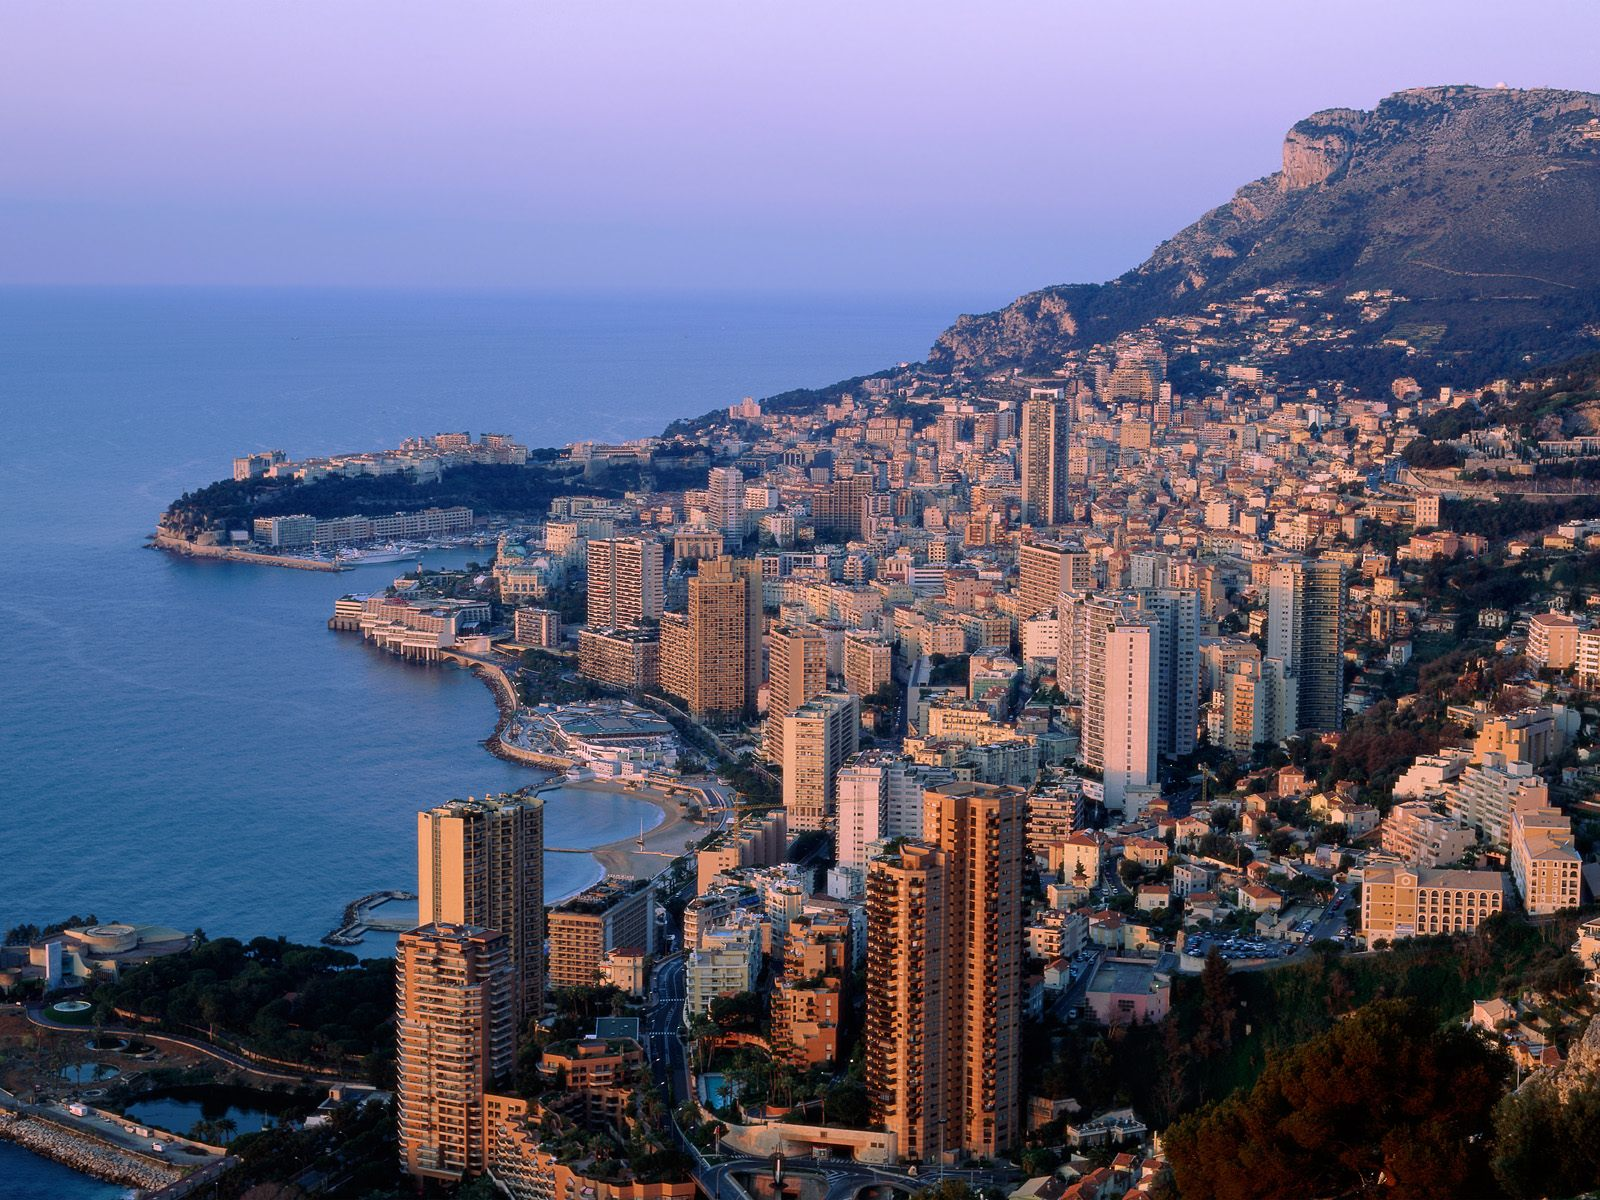
\includegraphics[scale=0.15]{MonteCarlo.jpg} 
\caption{Monte Carlo city}
\end{figure}
\end{frame}

\begin{frame}\frametitle{Stochastic systems modeling and analysis}
\begin{enumerate}
\item Queueing theory\pause 
\item Mathematical finance\pause 
\item Actuarial science\pause 
\item Physics
\end{enumerate}
\end{frame}

\begin{frame}\frametitle{Decision theory (matrix games)}
\begin{figure}
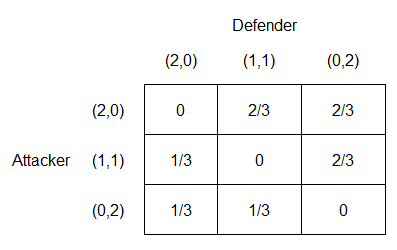
\includegraphics[scale=0.9]{MatrixGame.png} 
%\caption{War task}
\end{figure}
\only<2>{
Strategy = $\br{p_1, \quad, p_2, \quad p_3}$
}
\end{frame}

\begin{frame}\frametitle{Aesthetics}
\begin{figure}
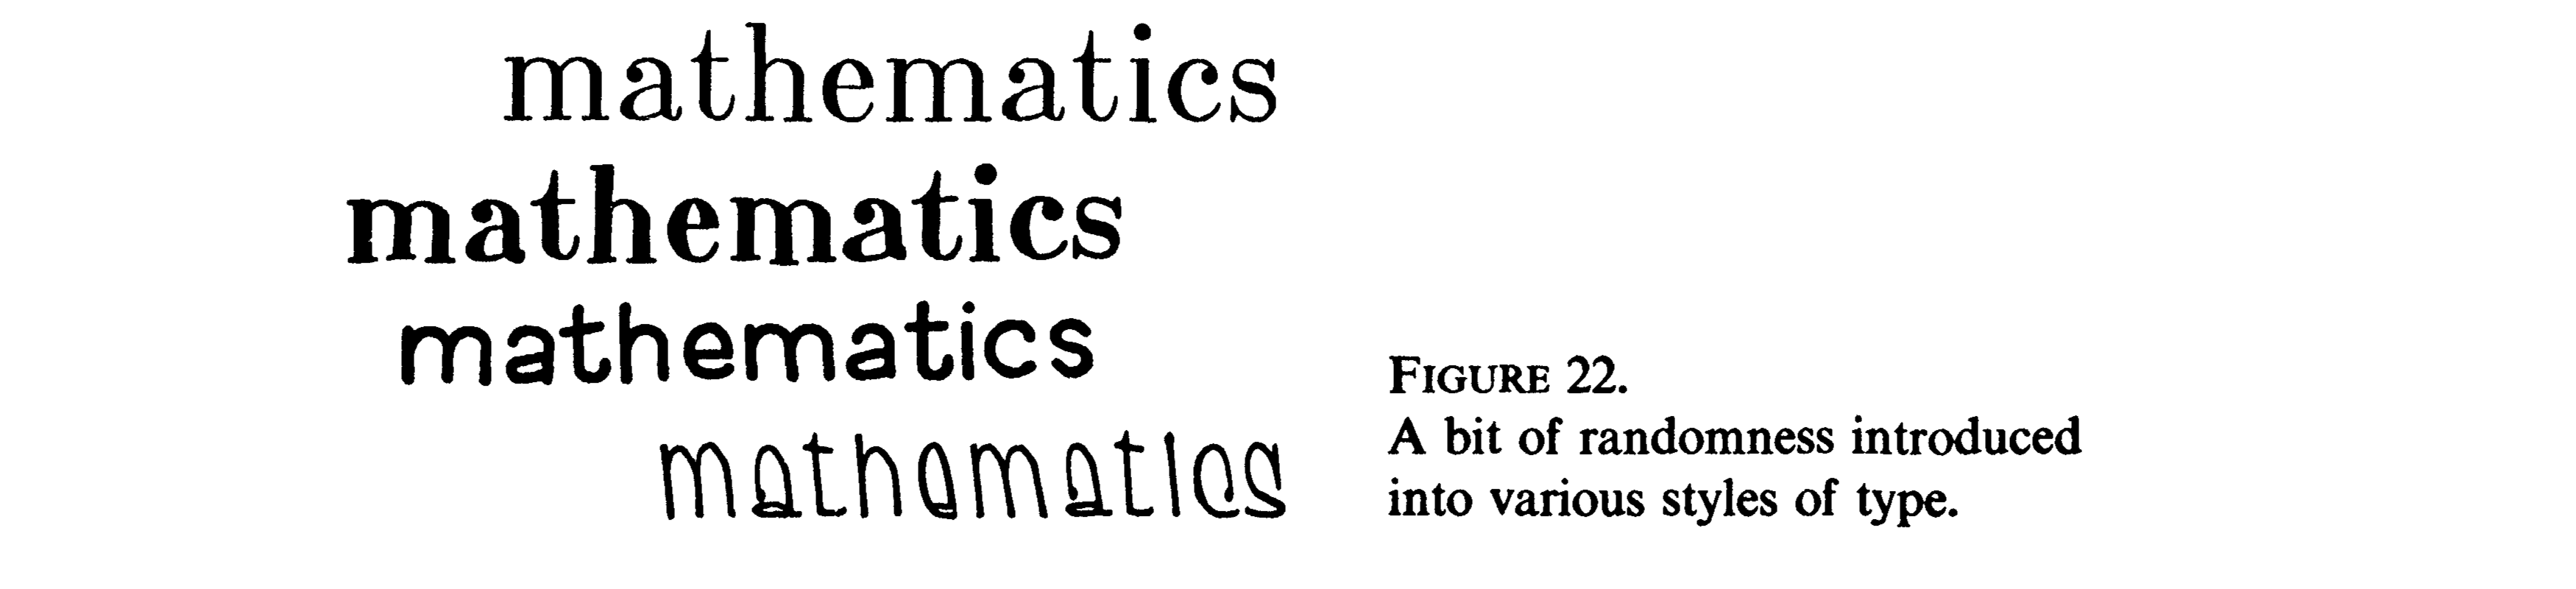
\includegraphics[scale=0.1]{Aesthetics.png} 
\end{figure}
``I think it can be said that the letters in this final example have a warmth and charm which makes it hard to believe that they were really 
generated by a computer following strict mathematical rules.''
\begin{flushright}
 {\small 
 D.E. Knuth, Mathematical typography --- Bull.  Amer. Math. Soc. 1 (1979), 369
 }
\end{flushright}

\end{frame}



\begin{frame}\frametitle{Numerical analysis}
{\small
Denote $f(y) = \sum_{i=1}^{n} y_i^2$.
Want to estimate
$$I = \int_{0}^1 dy_1\ldots \int_{0}^1 f(y)dy_n$$
with estimators ($N=M^n$):
$$\tilde{I}_1 = \frac{1}{N} \sum_{j=1}^N f(\overline{x}_j),$$
where $\brrr{\overline{x}_j}_{1\leqslant j\leqslant N}$ form uniform grid in $[0;1]^n$ cube
and
$$\tilde{I}_2 = \frac{1}{N} \sum_{j=1}^N f(\overline{x}^{'}_j),$$
where $\overline{x}^{'}_j$ is uniform random point in $j$-th subcube.
}
\end{frame}
\begin{frame}\frametitle{Numerical analysis}
{
\footnotesize
\begin{columns}
\begin{column}{5cm}
\begin {table}[h]
\caption{n=1}
\begin{center}
\begin{tabular}{| c | c | c |}
\hline 
N & $|I-\tilde{I}_1 |$ &  $|I-\tilde{I}_2|$\\
\hline
$ 10^2$ & $ 5*10^{-3}$ & $7*10^{-6}$\\
\hline
 $10^3$ &  $5*10^{-4}$ & $4*10^{-7}$\\
\hline
 $10^4$ & $ 5*10^{-5}$ & $5*10^{-9}$\\
\hline
 $10^5 $& $ 5*10^{-6}$ &$ 4*10^{-10}$\\
\hline
 $10^6 $&  $5*10^{-7}$ & $1*10^{-11}$\\
\hline
$10^7$ &  $5*10^{-8} $& $1*10^{-12}$ \\
 \hline
\end{tabular}
\end{center}
\end{table}
\end{column}

\begin{column}{5cm}
\begin {table}[h]
\caption{n=2}
\begin{center}
\begin{tabular}{| c | c | c |}
\hline 
N & $|I-\tilde{I}_1 |$ &  $|I-\tilde{I}_2|$\\
\hline
$10^2$ & $10^{-1}$& $ 6*10^{-5}$\\
\hline
$10^4$ & $10^{-2}$ & $ 10^{-6}$\\
\hline
$10^6$& $10^{-3}$&$5*10^{-7}$\\
\hline
$10^8$ &$10^{-4}$&$ 3*10^{-9}$\\
\hline
\end{tabular}
\end{center}
\end{table}
\begin {table}[h]
\caption{n=3}
\begin{center}
\begin{tabular}{| c | c | c |}
\hline 
N & $|I-\tilde{I}_1 |$ &  $|I-\tilde{I}_2|$\\
\hline
$10^3$& $0.145$& $2*10^{-3}$\\
\hline
$10^6$&$0.0145$&$ 6*10^{-6}$\\
\hline
\end{tabular}
\end{center}
\end{table}
\end{column}
\end{columns}

}
\end{frame}

\begin{frame}\frametitle{Numerical analysis}
Assume $f(\cdot)$ and $\frac{\partial f}{\partial x_k}$ are continuous and 
$\left|\frac{\partial f}{\partial x_k}\right| \leqslant L$, $1 \leqslant k \leqslant n$.

Then
\begin{block}{Assertion 1}
$$P\br{\left|I-\tilde{I}_2 \right| \leqslant (nL/\varepsilon) N^{-1/2 - 1/n}} \geqslant 1- \varepsilon^2, \quad0 < \varepsilon < 1$$ 
\end{block}
and
\begin{block}{Assertion 2}
$\sup_{f}\left|I-\tilde{I}_1 \right| \leqslant n L N^{- 1/n}$
\end{block}
\end{frame}

\subsection*{Descrete mathematics (algorithms)}
\begin{frame}[fragile] \frametitle{Quick sort}
Consider array $$\br{a[1], a[2], \ldots, a[N]}.$$ We want to sort it in direct (increasing) order.
{
\scriptsize
\begin{columns}
\begin{column}{5cm}
\begin{verbatim}
  // begin with QuickSort(a, 1, N)
  QuickSort(a, begin, end) 
  if begin < end
    then q = Partition (a,begin, end); 
    QuickSort(a, begin, q-1);
    QuickSort(a, q+1, end);
\end{verbatim}
\end{column}

\begin{column}{5cm}
 \begin{verbatim}
 Partition(a,begin,end)
  x = a[end];
  i = begin - 1;
  for j = begin to (end - 1)
    if a[j] <= x
      then i = i+1;
      exchange a[i] and a[j]
  exchange a[i+1] and a[end];
  return i + 1;
\end{verbatim}
\end{column}

\end{columns}
}
\end{frame}

\begin{frame}[fragile] \frametitle{Quick sort}
{
\small
$T(N) = ?$
{
\scriptsize
\begin{verbatim}
  // begin with QuickSort(a, 1, N)
  QuickSort(a, begin, end) 
  if begin < end
    then q = Partition (a,begin, end);  // (end - begin) <= (N - 1) iterations
    QuickSort(a, begin, q-1);           // T(q -  begin) <= T(N - 1) iterations
    QuickSort(a, q+1, end);             // T(end - q) <= T(N - 1) iterations
\end{verbatim}
}
In the worst case $$T(N) = (N-1) + (N - 2) + \ldots + 2 + 1 = \frac{(N -2)* (N-1)}{2} = O\br{N^2}$$ 
iterations when 
$$a[1] < a[2] < \ldots < a[N].$$
}
\end{frame}

\begin{frame}{Quick sort}
But! If 
$$P\br{a[i_1] < a[i_2] < \ldots < a[i_N]} = \frac{1}{N!}$$ for any permutation $(i_1,i_2,\ldots,i_N),$
then
$$\overline{T}(N) = E\brr{T(N)} = O\br{N \log{N}}!$$
\only<2,3>{
And what if instead of $\frac{1}{N!}$ we have arbitrary distribution
$$\br{p_1, p_2, \ldots, p_{N!}}?$$}
\only<3>{
Lets use pseudorandom numbers!
$$\overline{T}(N) = O\br{N \log{N}}.$$
}
\end{frame}

\begin{frame}{Matrix equations}
{
\small
 $A$, $B$ and $C$ $\in R^{N\times N}$.
 
 \begin{equation}
A\times B = C ?
\label{matrices}
 \end{equation}

Complexity (determined algorithms): $O\br{N^3}$ or $O\br{N^{2.3}}$.
 
\only<2,3>{
 $x\in \brrr{0;1}^N$ --- uniform random vector. Instead of \eqref{matrices} check
 \begin{equation}
A\times B \times x = C \times x ?  
\label{matricesOne}
 \end{equation}
Decision rule: if (2) is true (false) then \eqref{matrices} is true (false).  
}

\only<3>{
Complexity: $O\br{N^2}$. Error probability:
$$P\br{\text{"false"}|A\times B = C} = 0, \quad P\br{\text{"true"}|A\times B \neq C} \leqslant \frac12$$

Repeat it $20$ times and get error probability $< 10^{-6}$.
}
}
\end{frame}

\begin{frame}{Integer equations}
Let $x_1$, $x_2$, $\ldots$, $x_N$ $\in$ $Z_+$ and $Q\br{x_1,x_2,\ldots, x_N}$ be $k$-degree polinom.
 \begin{equation}
 Q\br{x_1,x_2,\ldots, x_N} \equiv 0 ?
  \label{equ}
 \end{equation}
 No polinomial algorith.

\end{frame}

\begin{frame}{Integer equations}
 
 \begin{block}{Shwartz Lemm}
  If $\brrr{x_i}_{1\leqslant i \leqslant N}$ are independent uniform random numbers from $\brrr{0, 1, \ldots, n}$
  then $$P\br{Q\br{x_1,x_2,\ldots, x_N} = 0 | Q\br{\cdot,\cdot,\ldots, \cdot} \not\equiv 0} < \frac{k N}{n}.$$
 \end{block}
 Let $n = 2 k N + 1$ then $P\br{\text{Error}} <1/2$.
 
 Check $100$ times => $P\br{\text{Error}} < {1/2^{100}}$
\end{frame}

\section{What does it mean <<random numers>>?}
\subsection{Problem formalization}
\begin{frame}{What does it mean <<random numbers>>? }
 \begin{figure}
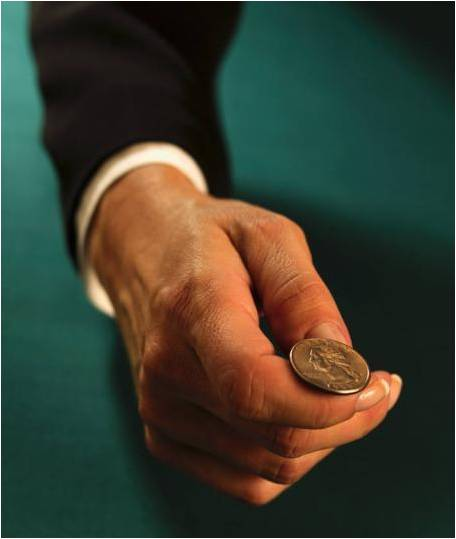
\includegraphics[scale=0.5]{coin-flip.jpg} 
\end{figure}
\end{frame}


\begin{frame}{Psychological test}
 \begin{align}
  1 0 0 0 1 0 1 1 1 0 1 1 1 1 0 1 0 0 0 0 \\
   0 1 1 1 1 0 1 1 0 0 1 1 0 1 1 1 0 0 0 1
   \nonumber
 \end{align}

\only<2>{
\begin{align}
 0 0 0 0 0 0 0 0 0 0 0 0 0 0 0 0 0 0 0 0\\
 1 1 1 1 1 1 1 1 1 1 1 1 1 1 1 1 1 1 1 1
 \nonumber
\end{align}
}
\end{frame}

\begin{frame}{}
Remarks: 
 \begin{itemize}
  \item $P\br{\xi_i = 1} = P\br{\xi_i = 0} = \frac12$
  \pause
  \item Consider only $\br{\xi_1, \xi_2, \ldots, \xi_N}$, where $N$ is large ($N\rightarrow \infty$)
 \end{itemize}

 
 \only<3>
{\begin{block}{Problem}
Denote $$\Omega = \brrr{0,1}^{\infty}.$$ 
Want to find $$R \subset \Omega \text{ --- set of random sequences.}$$
\end{block}
}
\end{frame}

\begin{frame}{General approach}
 Let $L\colon \Omega \rightarrow \brrr{0,1}$ be a characteristic property indicator of sequence $\br{a_1, a_2, \ldots}$. 
 \newline
 %
 \newline
 $\br{a_1, a_2, \ldots}$ --- random sequence $\Leftrightarrow$ $L\br{a_1, a_2, \ldots}=1$
 \newline
 %
 \newline
 %
 \newline
 \only<2>
 {
 \textcolor{blue}{What L functions can you imagine?}}
\end{frame}

\subsection{Definition 1. Frequency stability}
\begin{frame}{Intuitive assumption}
Consider sequence $$\br{a_1, \quad a_2,\quad  \ldots,\quad  a_{N-1},\quad  a_N,\quad  a_{N+1}, \dots}.$$
 Obviously we want
\textcolor{blue}{
\begin{equation}
  \lim_{N \rightarrow \infty} \frac{\nu_N\br{\text{"1"}}}{N} = \frac12,
 \end{equation}
 }
 where $\nu_N\br{\text{"1"}} = \sum_{i = 1}^N Indicator\brrr{a_i = 1}$.
\newline
%
\newline
\only<2>{
\textcolor{blue}{What about sequence $$0\ 1\ 0\ 1\ 0\ 1\ 0\ 1\ \ldots\ ? $$}
}
 
\end{frame}

\begin{frame}{Definition 1}
 \begin{block}{}
 $\br{a_1, a_2, \ldots}$ is random if for any computable functions $F()$ and $G()$:
  \begin{enumerate}
  \item $n(1) = F(\Lambda), n(2) = F(a_{n(1)})$
  $$\br{a_{n(1)}, a_{n(2)}, \ldots} \text{ -- mixed}$$
  \item Get $a_{n(k)}$ $\Leftrightarrow$ $G(a_{n(1)}, a_{n(2)}, \ldots, a_{n(k-1)}) = 1$
  $$(\tilde{a}_1, \tilde{a}_2, \ldots) \text{ --- result sequense}$$
  \end{enumerate}
true following $$\lim_{N \rightarrow \infty} \frac{\nu_N\br{\text{"1"}}}{N} = \frac12$$  
 \end{block}

\end{frame}


 \subsection{Definition 2. Unpredictability}
 \begin{frame}{Intuitive assumption}
 Let $$\br{a_1, a_2, \ldots}$$ be a casino tool, that is gamer tries to predict these numbers.
 \begin{enumerate}
  \item Gamer knows nothing and he just predicts $\br{n(1), i(1), v(1)}$; casino checks whether $i(1) = a_{n(1)}$; $V(1) = V(0) +/- v(1)$;
  \item Gamer knows $a_{n(1)}$ and tries to predict the next number; he says $\br{n(2), i(2), v(2)}$; $V(2) = V(1) +/- v(2)$;
  \item $\ldots$
 \end{enumerate}
Every time gamer applies some decision function $\Xi()$, named ``strategy''.
 \end{frame}
 
 \begin{frame}{Definition 2}
  Suppose gamer has $V(0) = 1$ money initially.
  \begin{block}{Definition}
   $\br{a_1, a_2, \ldots}$ is random if there is no computable strategy $\Xi()$, that implies 
   $$V(k) \xrightarrow[k \to \infty]{}  \infty.$$
  \end{block}
  
  \begin{block}{Theorem}
  Let $U$ be class of <<unpredictable>> sequences and $S$ be class of frequency stable sequences. 
  Then $$U \subset S.$$
  \end{block}
\end{frame}

\section{Pseudorandom numbers}

\subsection{Random and pseudorandom numbers}
\begin{frame}{Random and pseudorandom numbers}
\begin{columns}
 \begin{column}{5cm}
 \begin{figure}
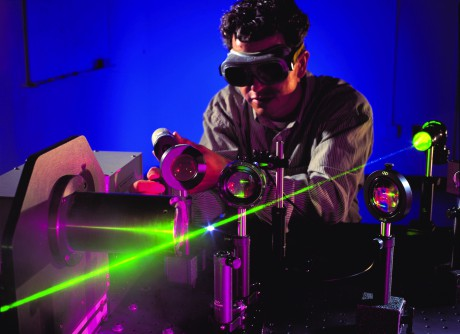
\includegraphics[scale=0.3]{RandExper.jpg} 
\caption{Random}
\end{figure} 
 \end{column}
 \begin{column}{6cm}
 \newline
 %
 \newline
 
\begin{figure}
   $$X_{n+1} = \br{a X_{n} + c} \mod m$$
\caption{ Pseudorandom}
\end{figure}
\end{column}


\end{columns}
 \end{frame}
 
 
  
 \subsection{Random numbers sources}
 \begin{frame}{Examples}
 \begin{itemize}
  \item Flipping a coin or dices, dragging balls from an urn etc; 
  \pause
  \item making radioactive decay experiments;
  \pause
  \item on Linux (v. $\geqslant 1.3.30$) reading \textit{/dev/random} file.
 \end{itemize}
 \end{frame}
 
 \begin{frame}{Disadvantages}
  \begin{enumerate}
   \item Slowness;
   \pause
   \item lack of replicability;
   \pause
   \item systematic bias.
  \end{enumerate}

 \end{frame}

\begin{frame}{Ways to improve}
  \begin{enumerate}
   \item Slowness \textcolor{blue}{(prerecorded tables)};
   \pause
   \item lack of replicability \textcolor{blue}{(prerecorded tables)}; 
   \pause
   \item systematic bias \textcolor{red}{(difficult to quantify, no general solution)}.
  \end{enumerate}
  \end{frame}

\begin{frame}{Advantages}
They are truly random! Nobody can argue with it.
\newline
%
\newline
\textcolor{blue}{Application:} as a seed for pseudorandom numbers.
 \end{frame}

 \subsection{Pseudorandom numbers sources}
 \begin{frame}{The first pseudorandom numbers generator}
  \begin{block}{John von Neumann.}
   Suppose we have $X_n$. Calculate $X_n^2$ and get, for example, 10 digits from the middle as $X_{n+1}$. 
  \end{block}
  Example:
  $$X_n = 5772156649 \rightarrow X_n^2 = 33317\textcolor{red}{7923805949}09201$$
  $$X_{n+1} = 7923805949$$
  \only<2>{
  Disadvantage: a few numbers and hard to calculate.
  \begin{block}{Assertion}
   20-digits binary number generates at maximum 142 different numbers.
  \end{block}
  }
  \end{frame}
  \begin{frame}{}
  ``Random numbers should not be generated with a method chosen at random''
\begin{flushright}
 {\small 
 D. E. Knuth ``The Art of Computer Programming'', 2, page 6
 }
\end{flushright}
\only<2>{
  \textcolor{blue}{Some theory should be used.}
  }
 \end{frame}

 \begin{frame}{What numbers do we need?}
  \begin{itemize}
   \item Every random number $U_n$ uniformly distributed in $\brr{0, 1}$ can be transformated to arbitrary distributed random number.
  \only<2,3>{
  \item Every number in a computer is represented with only finite accuracy.
  }
  \end{itemize}
  \only<3>{
  \begin{block}{General approach}
  $$ X_n \in \brrr{0, 1, \ldots, m - 1} \rightarrow U_n = X_n/m \rightarrow \textit{ arbitrary distribution}$$
  \end{block}
  Hence we need $X_n \in \brrr{0, 1, \ldots, m - 1}$.
  }
 \end{frame}

 \subsection{The Linear Congruential Method}
\begin{frame}{Definition}
Choose four numbers:
 \begin{itemize}
  \item $m$ --- the modulus; $0 < m$.
  \item $a$ --- the multiplier; $0 \leqslant a < m$.
  \item $c$ --- the increment; $0 \leqslant c < m$.
  \item $X_0$ --- the starting value; $0 \leqslant X_0 < m$
 \end{itemize} 
 
 %
\only<2>{
$$X_{n+1} = \br{a X_n + c} \mod m, \quad n \geqslant 0.$$
}
 \end{frame}
\begin{frame}{Example}
 For $m = 10$, $X_0 = a = c = 7$ we get
 $$7,\ 6,\ 9,\ \textcolor{red}{0},\ 7,\ 6,\ 9,\ \textcolor{red}{0},\ \ldots$$
Congruential sequences always get into loop. Unfortunately.
\end{frame}


 \begin{frame}{Choise of modulus ($m$). {\normalsize $X_{n+1} = \br{a X_n + c} \mod m$}}
  \begin{itemize}
   \item \textcolor{blue}{Period length $< m$.}
   
   \only<2,3>{
   \item \textcolor{blue}{Generation speed.}
   
   Using $m = 2^e$ numbers ($e$ is a computer's word size, e.g.) is faster.
   }
   \only<3>{
   \item \textcolor{blue}{Random properties.}
   
   Suppose $m = 2^e$ $\Longrightarrow$ the right-hand digits of $X_n$ are much less random than the left-hand digits.
   \begin{block}{Assertion}
    If $d$ is divisor of $m$ and if $\br{Y_n = X_n \mod d}$ then $$Y_{n+1} = \br{a Y_n + c} \mod d.$$
   \end{block}
  You can use $m = 2^e -1$ instead.
  }\end{itemize}
 \end{frame}
\begin{frame}{Choise of multiplier ($a$) and increment ($c$). {\normalsize $X_{n+1} = \br{a X_n + c} \mod m$}}
 \textcolor{blue}{Goal:} achieve the longest period ($m$). Is it possible?
 \only<2,3>{
 
 \textcolor{blue}{Yes:}$$  X_{n+1} = \br{X_n + 1} \mod m.$$
 }
 \only<3>{
 \begin{block}{Theorem}
  The linear congruential sequence defined by $m$, $a$, $c$ and $X_0$ has period length $m$ if and only if
  \begin{enumerate}
   \item $c$ is relatively prime to $m$;
   \item $a - 1$ is a multiple of $p$, for every prime $p$ dividing $m$;
   \item $a - 1$ is a multiple of $4$, if $m$ is a multiple of $4$.
  \end{enumerate}
\end{block}
 }
\end{frame}

\subsection{Randomness criterias}
\begin{frame}{Potency. {\normalsize $X_{n+1} = \br{a X_n + c} \mod m$}}

 Suppose $\brrr{X_n}$ has maximum period (that is $m$).
 \begin{block}{Definition}
  The least integer $s$ such that $$\br{a-1}^s \equiv 0 \br{\textit{ modulo }m}$$
  called <<potency>>.
 \end{block}
 
 The larger potency $\Longrightarrow$ the more random sequence.
% 
\end{frame}
 
 \begin{frame}{Potency. {\normalsize $X_{n+1} = \br{a X_n + c} \mod m$}}
 {\normalsize
  Let $X_0 = 0$ and $b = a - 1$, then 
  $$X_n = \br{\br{a^n - 1}c/b} \mod m,$$
  after transformations:
  $$X_n = c\br{n + {{n}\choose{2}} b + \ldots + {{n}\choose{s}} b^{s-1}} \mod m.$$
  \only<2,3>{
  \textcolor{blue}{In particular:}
  
  $s = 1 \Longrightarrow X_n = cn \mod m;$
  
  $s = 2 \Longrightarrow X_n = c n + c {{n}\choose{2}}b \mod m$ $ \Longrightarrow  X_{n+1} - X_n\equiv c + c b n $
  \only<3>{
  %\scriptsize
  \par \ \ \  denoting $\br{d = cb \mod m}$ we have $\br{X_n, X_{n+1}, X_{n+2}} \in $
  \begin{align*}
  x - 2y + z &= d + m , &x - 2y + z &= d - m,\\
  x - 2y + z &= d, &x - 2y + z &= d - 2m.\\
\end{align*}
}
  }
  }
 \end{frame}

 \begin{frame}{Potency. {\normalsize $X_{n+1} = \br{a X_n + c} \mod m$}}
 \textcolor{blue}{Examples:}
 \begin{enumerate}
  \item Let $m = 2^e$; it is divisible by high powers of prime $2$. Choosing $a = 2^k + 1$, have relatevely big potency.
 \only<2>{
 \item Let $m = 2^e - 1$; commonly it is \textcolor{red}{not} divisible by high powers of primes $\Longrightarrow$. There could not be a big potency.
 }
 \end{enumerate}
  
 \end{frame}
 
 \begin{frame}{"Chi-square" test. Experiment}
 Throw two "true" dices.
 
 $s$ --- sum of the result numbers.
 \begin {table}[h]
\begin{center}
\begin{tabular}{|  c | c | c | c | c | c | c | c | c | c | c | c |}
\hline
 value of $s = $ & 2 & 3 & 4 & 5 & 6 & 7 & 8 & 9 & 10 & 11 & 12\\
 \hline
 probability, $p_s  = $ & $\frac{1}{36}$ & $\frac{1}{18}$ & $\frac{1}{12}$ & $\frac{1}{9}$ & $\frac{5}{36}$ & $\frac{1}{6}$ & 
 $\frac{5}{36}$ & $\frac{1}{9}$ & $\frac{1}{12}$ & $\frac{1}{18}$ & $\frac{1}{36}$ \\
 \hline
\end{tabular}
\end{center}
\end{table}

\only<2>{
Repeat $n=144$ times:
 \begin {table}[h]
\begin{center}
\begin{tabular}{| p{2.8 cm} | c | c | c | c | c | c | c | c | c | c | c |}
\hline
 \small value of $s = $ & 2 & 3 & 4 & 5 & 6 & 7 & 8 & 9 & 10 & 11 & 12\\
 \hline
 observed \par number, $Y_s = $ & 2 & 4 & 10 & 12 & 22 & 29 & 21 & 15 & 14 & 9 & 6 \\
 \hline
 probability, $p_s  = $ & $\frac{1}{36}$ & $\frac{1}{18}$ & $\frac{1}{12}$ & $\frac{1}{9}$ & $\frac{5}{36}$ & $\frac{1}{6}$ & 
 $\frac{5}{36}$ & $\frac{1}{9}$ & $\frac{1}{12}$ & $\frac{1}{18}$ & $\frac{1}{36}$ \\
 \hline
\end{tabular}
\end{center}
\end{table}
}
 \end{frame}
 
\begin{frame}{"Chi-square" test. Statisctic}
 \begin{equation}
  V = \br{Y_2 - n p_2}^2 + \br{Y_3 - n p_3}^2 + \ldots + \br{Y_{12} - n p_{12}}^2.
 \end{equation}
\only<2,3>{
 Better to analyse:
 \begin{equation}
  V = \frac{\br{Y_2 - n p_2}^2}{n p_2} + \frac{\br{Y_3 - n p_3}^2}{n p_3} + \ldots + \frac{\br{Y_{12} - n p_{12}}^2}{n p_{12}}.
 \end{equation}
 }
 \only<3>{
 In our example:
 \begin{equation}
  V = \frac{\br{2 - 4}^2}{4} + \frac{\br{4 - 8}^2}{8} + \ldots + \frac{\br{9 - 8}^2}{8}  + \frac{\br{6 - 4}^2}{4} = 7 \frac{7}{48}.
 \end{equation}
 }
\end{frame}

\begin{frame}{"Chi-square" test. Test}
\footnotesize
 $$V = \sum_{s = 1}^k \frac{\br{Y_s - n p_s}^2}{n p_s}  \xrightarrow{d} \chi^2\br{k-1} $$
 \only<2>{
\begin{columns}
 \begin{column}{6cm}
 \begin{figure}	
 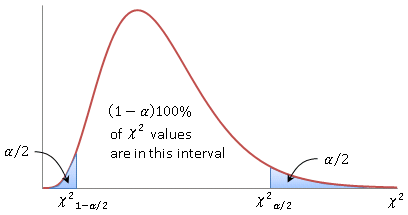
\includegraphics[scale=1.8]{chi-square-dist2.png} 
\caption{ $\chi^2\br{k-1}$ density}
\end{figure}
\end{column}
 \begin{column}{5cm}
  \begin{multline*}
P\left( \chi_{1 - \alpha / 2}^2\br{k-1} \leqslant \right. \\ \left. \leqslant V\br{Y_1, Y_2, \ldots, Y_k} \leqslant  \right. \\
\left. \leqslant \chi_{\alpha / 2}^2\br{k-1}
| V \in \chi^2\br{k-1}\right) =\\= 1 - \alpha
\end{multline*}
\end{column}

\end{columns}
}
\end{frame}

\begin{frame}{"Chi-square" test. Pseudorandom numbers generators app}
Consider
 $$A = \brrr{0, 1, \ldots, m - 1}.$$
 \only<2,3,4,5>
 {Split $A$ into $k$ subsets (of size $\frac{m}{k}$, e.g.):
 \begin{multline*}
A = \brrr{0, 1, \ldots, \frac{m}{k} - 1} \cup \brrr{\frac{m}{k},\frac{m}{k} + 1, \ldots, 2 \frac{m}{k} - 1} \cup \ldots \\
\ldots
 \cup \brrr{m - \frac{m}{k},m - \frac{m}{k} + 1, \ldots, m - 1}.
 \end{multline*}
 }
 \only<3,4,5>{
 Generate $n$ random numbers. $n$ should satisfy
 }
 \only<3>{
 $$n p_s = \frac{n}{k} \geqslant 5$$
 }
 \only<4>{
 $$n p_s = \frac{n}{k} \geqslant 5, \quad \text{ better }\quad \geqslant  8$$
 }
 \only<5>{
 $$n p_s = \frac{n}{k} \geqslant 5 \quad \text{ better}\quad \geqslant  8 
  \quad \text{ better }\quad \geqslant  10$$
 }
\end{frame}

\end{document}